%Group Report Information: How does your device work? Describe in as much detail as you can fit into the report. It should contain three subsections: Mechanics, Electronics and Software/Firmware. Describe also what alternatives you analyzed for the different parts of your device. Why did you select the alternative that you finally used?

\section{Description}
\begin{figure}[h]
\centering
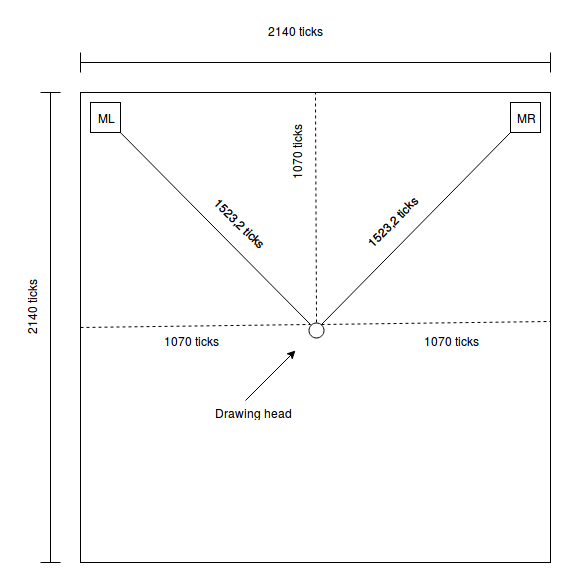
\includegraphics[scale=0.30]{Images/DrawingMachine/Illustration.png}
\caption{ Drawing machine concept. }
\label{OverviewFigure}
\end{figure}

\subsection{Design}
The designing phase of the Drawing Machine has been an iterative process going back and forth until a design was suitable enough for our requirements. Through the trial and error process we learned a lot about how to do better but in many cases also simpler. In some cases we ended up over-engineering solutions only to figure out it would make the whole machine much more complex and could be done much more simple.\\
Figure \ref{OverviewFigure} shows an overview of how we imagine our drawing machine to work. A motorbox is ML and MR on the figure. A box has a pianowire forming a loop to guide the wire from a spindle on a shaft of a stepper motor placed in the box. The loop will guide the wire from the middle of the spindle down to a part that has a hole towards and close to the whiteboard. This will keep the wire close to the whiteboard and it will be at this point that we say that there is a triangle between the motors and the drawing head. The wire will be pulled/released to move the drawing head. The drawing head is pulled down by gravity with the help of a weight.\\ The resulting design of the Drawing Machine is seen in appendix. The Drawing Machine's stepper motor is set inside two boxes that have nine magnet underneath.The boxes were designed in Fusion360 and then laser cut in a 6mm wooden plate\footnote{See appendix }.On the stepper motor we designed first a spindle in Fusion360 with the idea of solving an issue of the wire rolling onto itself. The result of the design is seen in appendix.... but the issue with this solution was the rotation of the spindle. It would draw on the wire and then release giving us a hard time to control. Instead we did a classic spindle design though with the issue of an error in diameter due to the wire rolling onto itself.\\
Next design part was the drawing head. It was important it was able to not only hold the pen but also push down the wire in order to be stable. we introduced a wooden block that kept our pen steady during drawing. In the beginning we discussed the possibility of the pen being lifted from the board during transport and then pushed to the board when drawing. Because of scope and our artistic interest we chose to let the transport lines be drawn and therefore let the pen stay in the same position all the time.  
\subsection{Mechanics}
The motors of the machine was originally intended to be placed with arbitrary length from one another, but lack of insight resulted in us not being able to assert the exact distance between the motors for an arbitrary setup. There had been ideas to include a load-cell or accelerometers to detect a tightened wire between the two motors. This could effectively have been used to assert the distance as a process of homing which results in the motors knowing how long the wire is from the given motor to the painting head.\\
This meant that for simplicity we assumed a fixed distance between the motors. {\it Homing} is then used to assert the length of the wire from the painting head, to a motor (ML or MR, see figure \ref{OverviewFigure}). This is done by placing a reed switch besides each motor such that the wire length will be the same when homing to either ML or MR, also it should home till the wire is as close to zero as possible. Both of these will affect accuracy.\\
The distance between ML and MR was measured to be 1070mm and as there are many triangles with two equally lengthen sides, we had to assume a length for the starting position after homing. We set this to 1070mm/2 = 535mm which placed the painting head pretty centered on our whiteboard. 

\subsection{Electronics}
The stepper motors used is model JK42HS34-1334 \footnote{For the lack of a datasheet, see \url{https://www.aliexpress.com/item/10-PCS-NEMA17-stepper-motor-3D-printer-stepper-motor-JK42HS34-1334A-30oz-in-34mm-1-3A/1571641221.html}}. This means that since the spindle on the motor is 2mm and the motor turns 1.8 degree each step, we have that $ (2*\pi*2)/360*1.8 = 0.06cm $, which means that the software will know the distance between ML and MR not as say 1070mm, but as $ 1070mm/0.6mm/step = 1783 steps $.\\
To control the stepper motors, we will be using two 
"Pololu - A4988 Stepper Motor" Drivers \citep{Pololu:StepperDriver}. These drivers can deliver 1A without a heat-sink. They are therefore needed as one of our stepper motors operate at 1.33A. We were especially made aware of this as the driver hit the 165 degree "Thermal Shutdown Temperature" feature of the driver that is mentioned in the datasheet. This caused noticeable loss of steps. Furthermore since we have two stepper motors, it amounts to over 2A which is the highest current-rated power-source we could acquire. This is however not a consistent load (its maximum), but this can be tolerated by setting the current limiter onboard the Polulu driver such that each stepper only draw 1A each.\\ 
To enable the drawing machine to home. The drawing head will have a magnet attached to the wire (same distance on each wire from the magnet to the drawing head). To enable the machine to know that this magnet reaches one of the motors ML or MR (see \ref{OverviewFigure}), there will be a reed switch placed at the end of the line near ML and MR. The electronics aspect of this is the reed switch as well as how to connect it. It is connected to a GPIO logic pin of the raspberry PI. Any input must have a pull-down resistor to ground aside from the sensor that switches positive power to the pin when triggered. This means that the input pin will either get a direction to ground or a direct connection to positive.\\
The complete schematic of connecting the polulu boards, steppers, reed switches and raspberry PI is shown in figure \ref{DrawingMachineSchematic}. Notice also how there is an electrolytic capacitor placed on the motor power source. This is to protect the board against LC voltage spikes \footnote{Polulu board product page. \url{https://www.pololu.com/product/1182}}. We found the driver broke sometimes and we therefore added it which fixed that reliability issue.  \\

\begin{figure}[h]
\centering
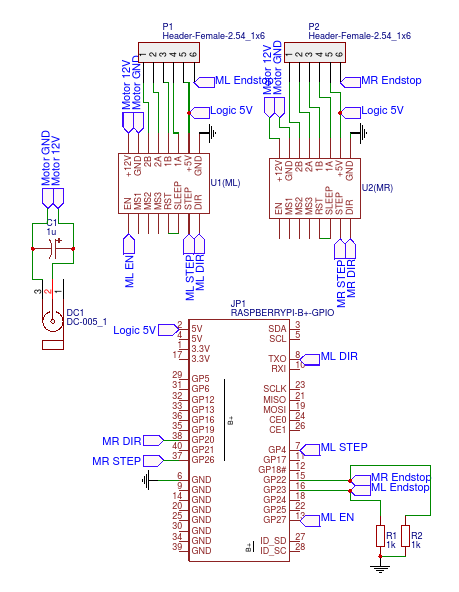
\includegraphics[scale=0.60]{Images/DrawingMachine/Schematic.png}
\caption{ Drawing machine electronics schematic. }
\label{DrawingMachineSchematic}
\end{figure}
 
If we know we want to draw a line from say (0,0) to (10,10), we have to consider that simply telling the motors to adjust their position for the correct line length isn't enough. There are many movements that could travel from A to B and thus to give the illusion of a straight line, we split a line between A and B into a number of coordinates along the line. The amount should just be relative to the resolution of the drawing machine which is 0.6mm per step. This is a problem to be fixed in the software/firmware section.

\subsection{Software/Firmware}
The software is written in python and is aimed at giving one Raspberry PI the capability to segment images into tracable ordered list of coordinates, act as controller for the motors, and to read input from the sensors. This section will describe the most essential aspects of each part.
\\\\
\subsubsection{Segmentation}
The segmentation logic is implemented in one encapsulating python class that takes as instantiating input a path to an image. All images are converted to their gray scale intensities using the {\it Python Image Library}(PIL)\footnote{\url{http://www.pythonware.com/products/pil/}}. Finding pixels to be colored is done using a threshold that defaults to $10$, thereby pixels, $p_{ij}$, are colored if the intensity of $p_{ij}$, $intensity_{ij}$, is such that:
\newline
$intensity_{ij} < threshold\ |\ {0 \leq i < 10, i \in \mathbb{N}}, $
\newline
where the possible intensities is in the range: $[0, 255]$.
For every pixel, $p_{ij}$ that matches this threshold, the segmentation will consider a neighborhood of the surrounding pixels. The size of the neighborhood greatly impacts the final result, since the drawing machine is not capable of lifting the drawing head from the board, and thus draws in one continuous line. This is seen from our simulated experiments with different neighborhoods shown in figure \ref{fig:simulating_experiments}. The simulation is made by plotting each point in an image using {\texttt PIL} rather than sending them as output to any motors. Thereby allowing us to make faster iterative adjustments.
The neighborhood dictates how many adjacent pixels are drawn before the scanning continues which manifests as a {\it transport line} on the final drawing between the last pixel to be colored in the current neighborhood and to the first pixel in the next. Too small of a neighborhood results in more transport lines since less pixels will be considered within the proximity to be drawn and so the scanning will continue to find another pixel to be colored, see figure \ref{subfig:3x3}. On the other hand, a too large neighborhood will result in too many pixels to be considered within the proximity of the currently scanned pixel, thereby the output may seem borderline abstract since otherwise distinct lines are considered the same, an example of this occurs in figure \ref{subfig:100x100}.
\begin{figure}[t]
\caption{Simulated experiments of different segmentation neighborhood sizes}
\label{fig:simulating_experiments}
    \begin{subfigure}[t]{.15\textwidth}
        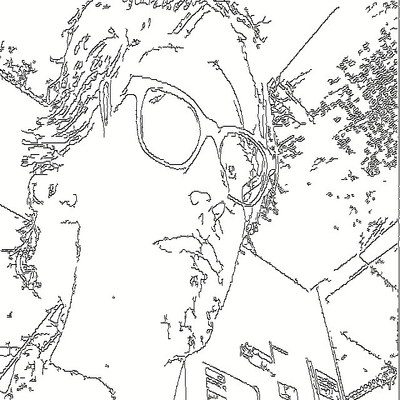
\includegraphics[width=\textwidth]{Images/original_input_resized_400x400.jpg}
        \caption{Original input resized to a fixed $400\times400$}
        \label{subfig:original}
    \end{subfigure}
    \begin{subfigure}[t]{.15\textwidth}
        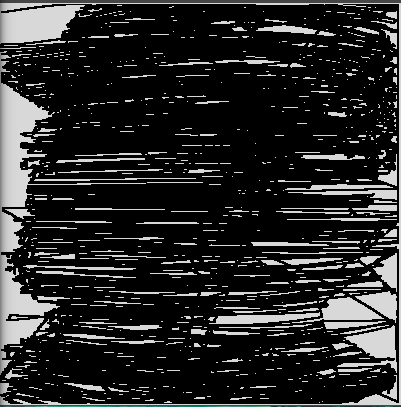
\includegraphics[width=\textwidth]{Images/segmented_v1_3x3_neighborhood.png}
        \caption{$3\times3$ neighborhood}
        \label{subfig:3x3}
    \end{subfigure}
    \begin{subfigure}[t]{.15\textwidth}
        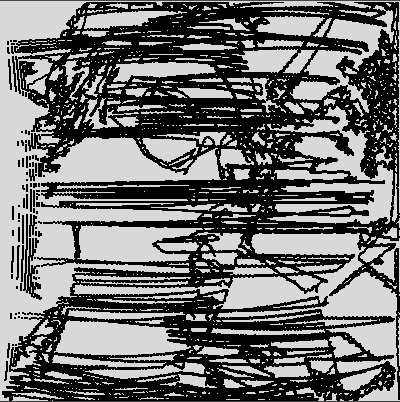
\includegraphics[width=\textwidth]{Images/segmented_v2_5x5_neighborhood.png}
        \caption{$5\times5$ neighborhood}
        \label{subfig:5x5}
    \end{subfigure}
    %next row:
    \begin{subfigure}[t]{.15\textwidth}
        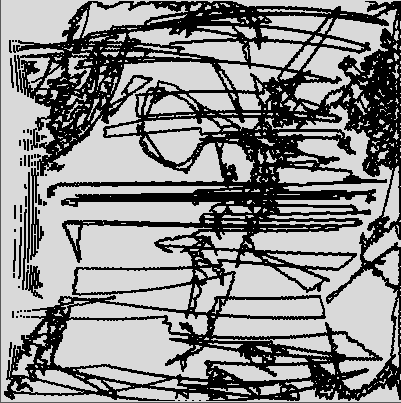
\includegraphics[width=\textwidth]{Images/segmented_v3_7x7_neighborhood.png}
        \caption{$7\times7$ neighborhood}
        \label{subfig:7x7}
    \end{subfigure}
    \begin{subfigure}[t]{.15\textwidth}
        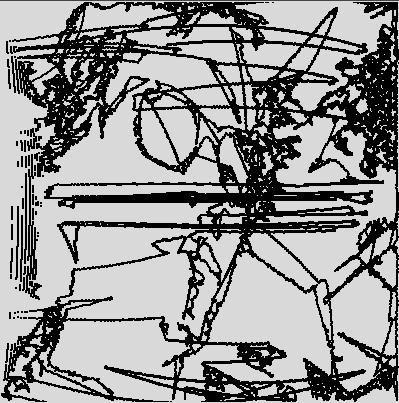
\includegraphics[width=\textwidth]{Images/segmented_v4_9x9_neighborhood.png}
        \caption{$9x9$}
        \label{subfig:9x9}
    \end{subfigure}
    \begin{subfigure}[t]{.15\textwidth}
        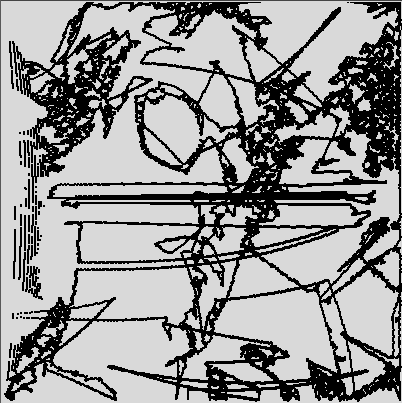
\includegraphics[width=\textwidth]{Images/segmented_v5_11x11_neighborhood.png}
        \caption{$11\times11$ neighborhood}
        \label{subfig:11x11}
    \end{subfigure}
    % last row:
    \begin{subfigure}[t]{.15\textwidth}
        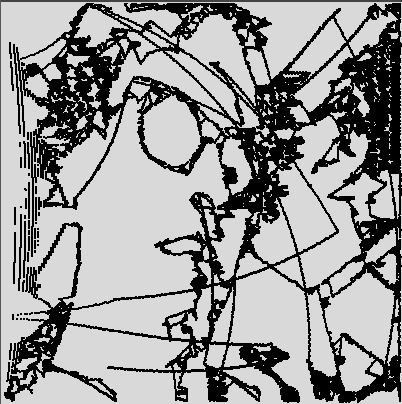
\includegraphics[width=\textwidth]{Images/segmented_v6_22x22_neighborhood.png}
        \caption{$22\times22$ neighborhood}
        \label{subfig:22x22}
    \end{subfigure}
    \begin{subfigure}[t]{.15\textwidth}
        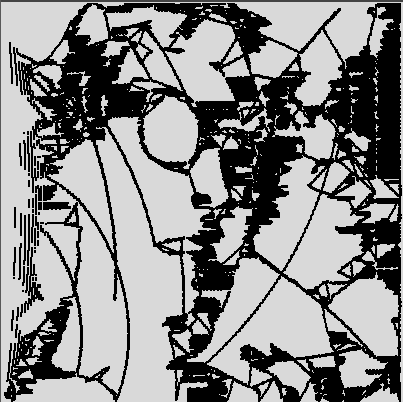
\includegraphics[width=\textwidth]{Images/segmented_v7_47x47_neighborhood.png}
        \caption{$47\times47$ neighborhood}
        \label{subfig:47x47}
    \end{subfigure}
    \begin{subfigure}[t]{.15\textwidth}
        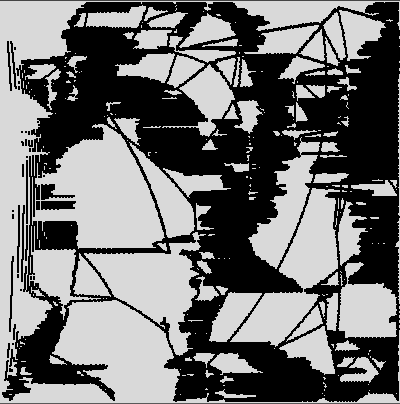
\includegraphics[width=\textwidth]{Images/segmented_v8_100x100_neighborhood.png}
        \caption{$100\times100$ neighborhood}
        \label{subfig:100x100}
    \end{subfigure}
    
\end{figure}

By default we set the size of the neighborhood to be considered a $11\times11$ matrix around the currently considered pixel. The reason for this default size was a trade-off between computation time and an optimal neighborhood size as judged by our simulations. As such, the neighborhood for pixel $p_{ij}$ are the pixels in $\big\{p_{i-2, j-2}, \dotsc, p_{i+2,j+2}\big\}$.
\\\\
\subsubsection{Auto calibration}
For autocalibration, two reed switches, one for each corner, was connected to the Raspberry Pi. The {\it homing} functionality would then first pull the motor up to one corner until the signal from the switch was sent to the Pi, then it would pull the motor to the second corner until a signal was received from the other switch. \\
At each signal, the line length of the corresponding motor was set to $0$. Thereafter, each motor, represented by an instance of a {\texttt Motor} class, is itself responsible for maintaining a counter of the current line length. For simplicity, the line length as well as the dimensions of the coordinate system itself, is measured in stepper motor {\it ticks}. That way, the logic for each motor class would only need to decrement or increment their counter based the direction parameter upon an invocation of their {\texttt tick} method.
\\\\
The implementation for the calibration functionality is largely simplified as two consecutive while loops that is set to continue for as long as no signal is received. Though, one obstacle was that we found that noise could influence a false positive signal being sent prematurely, and so we tackled this logically, by defining the constrain for the {\it while} loops to read $4$ consecutive signals. This approach proved sufficient to filter out false positives signals from the reed switches. 

\subsubsection{Motor control}
The motor control is based on inputs being given as $(x,\ y)$ coordinates and then translating these coordinates into corresponding line length. At the same time, two instantiations of a motor class, as mentioned in the previous section, represents the state of each motor and maintains a counter of the current line length of each line. Given an input $(x,\ y)$ of a desired coordinate to move to, length of the lines $left$ and $right$ is computed as two triangles respectively. That is,
\begin{align}
left  &= \sqrt{x^2 + y^2} \\
right &= \sqrt{(width-x)^2 + y^2} 
\end{align},
for line length {\it left} and {\it right}.
\\\\
After the desired line length is computed, the absolute difference between the current line length of {\it left} and {\it right} and their desired length, is used to know the relative speed needed in order for both adjustments to occur simultaneously.\\
The first iteration of our code, attempted to accommodate for this simultaneous movement through pythons {\it subprocess} library, and then having the motors to be responsible of the delay between each {tick} so that the arrival would match. However, this did not work very wel due to the asynchronous nature of this approach. The {\texttt time.sleep}, which ultimately leaves the scheduling of the frequency of ticks to the operating system to adhere to, was much too imprecise.
\\\\
In the end, everything is run as the same process, and both motors are controlled via the same {\it while} loop. A timestamp is assigned to each motor which is updated everytime a motor is asked to {\it tick}. Then comparing the timestamp for each motor with the current, the motor is asked to move when the frequency, measured in time, is smaller than the time delta. To avoid rounding errors, a method, {\it approx}, is used to measure whether the current line length is within one tick of the desired length. This prevents to motor going on endlessly moving back and forth.

% \begin{figure}
% \begin{python}
% def getNextLineLength(self, next_pos):                                                                             
%     """ Given the next coordinate set, next_pos,                                                   
%         compute the lenght of the line for motorRight                                         
%         and motorLeft                                    
%     """                                                                
%     x, y = next_pos                                                                              
%     # compute left triangle:                                                                  
%     left  = math.sqrt(x**2 + y**2)                                                         
%     # compute right triangle:                                                   
%     right = math.sqrt((self.width - x)**2 + y**2)

%     return left, right
% \end{python}
% \caption{Code snippet showing the computation of next line length given a coordinate set, {\it next\_pos}}
% \label{fig:compute_line_length_code}
% \end{figure}